%----------------------------------------------------------------------------------------
%	SECTION 1.1
%----------------------------------------------------------------------------------------

\section{Connected Spaces of The Real Line.}

\begin{definition}
    We call a simply ordered set $L$ with  $|L|>1$ a  \textbf{ordered contunuum} if:
        \begin{enumerate}
            \item[(1)] $L$ has the least upperbound property.

            \item[(2)] If $x<y$, then there exists a  $z$ such that  $x<z<y$.
        \end{enumerate}
\end{definition}

\begin{theorem}\label{3.2.1}
    If $L$ is a linear continuum in the order topology, then  $L$ is connected, and so are the open
    sets of  $L$  (the intervals and rays in $L$).
\end{theorem}
\begin{proof}
    We show that convex sets are connected. Let $Y=A \cup B$ be a seperation, and choose  $a \in A$,
     $b \in B$ with  $a<b$. We have that the interval of points in  $L$,  $[a,b] \subseteq Y$; and
     we also have that $[a,b] \subseteq A_0 \cup B_0$ with $ A_0=A \cap [a,b]$ and $ B_0=B \cap
     [a,b]$. Now $ A_0,B_0 \neq \emptyset$, so $[a,b]=A_0 \cup B_0$ is a seperation of $[a,b]$. Now
     let $c=\sup{A_0}$. Suppose first that $c \in B_0$, then $c \neq a$, so either $c=b$ or  $a<c<b$.
     Since  $ B_0$ is open in $[a,b]$ as a subspace of $Y$, there is some interval  $(d,c] \subseteq
     B_0$.

     If $c=b$, then  $d<c$ is an upperbound of  $ A_0$, which contradicts that $c$ is the least
     upperbound. Now suppose that $c<b$. We have that since  $c,b \in B_0$, $(c,b] \cap A_0=
     \emptyset$, then $(b,d] \cap A_0=(d,c] \cap (c,b] \cap A_0 = \emptyset$, and again we have
     $d<c$ which gives us the contradiction. So  $c \notin B$. By similar reasoning  $c \notin A_0$.
\end{proof}
\begin{corollary}
    $\R$ is connected and so are the intervals and rays of  $\R$.
\end{corollary}
\begin{proof}
    $\R$ is a linear continuum.
\end{proof}

\begin{theorem}[The Intermediate Value Theorem]\label{3.2.2}
    Let $f:X \rightarrow Y$ be continuous with  $X$ connected, and  $Y$ an ordered set under the
    order topology. If  $a,b \in X$, and if  $r \in Y$ such that  $f(a)<r<f(b)$ or $f(b)<r<f(a)$,
    then there exists a $c \in X$ for which  $f(c)=r$.
\end{theorem}
\begin{proof}
    Let $r \in Y$ such that  $f(a)<r<f(b)$, without loss of generality. We have that $A=f(X) \cap
    (-\infty, r)$ and $B=f(X) \cap (r ,\infty)$ are disjoint, nonempty sets open if $f(X)$ as a
    subspace of $Y$. Now suppose there is no  $c \in X$ for which  $f(c)=r$, then $f(X)=A \cup B$ is
    a seperation of $f(X)$, which contradicts theorem \ref{3.1.6}.
\end{proof}

\begin{example}
    \begin{enumerate}
        \item[(1)] The ordered square $I_0^2$ is a linear continuum. Let $A \subseteq I_0^2$ and consider
            the projection $\pi_1:I_0^2 \rightarrow I_0^2$. Let $b=\sup{\pi_1(A)}$, now if $b \in
            \pi_1(A)$ then $A \cap (b \times I_0) \neq \emptyset$, and since $I_0 \subseteq \R$, $A
            \cap (b \times I_0)$ has a least upperbound, $b \times c$, where  $c=\sup{I_0}$, which
            is also the least upperbound of $A$. Now if we have $a \times c < b \times d$, then
            $a<b$ and  $c<d$; and since  $\R$ is a linear continuum, there are $y,z \in \R$ for
            which  $a<y<b$ and  $c<z<d$. Hence  $a \times c < y \times z < b \times d$; which makes
            $ I_0^2$ into a linear continuum.

        \item[(2)] If $X$ is a well ordered set, then  $X \times [0,1)$ is a linear contiuum in the
            dictionary order. Let $A \subseteq X \times [0,1)$ and consider the projection $\pi_2:X
            \times [0,1) \rightarrow [0,1)$. If $b=\sup{\pi_2(A)}$, then $A \cap (b \times [0,1)) \neq
            0$, and so $A \cap (b \times [0,1)$ has a least upperbound $b \times c$ with
            $c=\sup{[0,1)}$, which is also a least upperbound of $A$.

            Now since $\R$ is a linear continuum, if $x \times a < y \times b$, under the dictionary
            order, then  $x \leq y$ and  $a<b$. Then there are  $c,z \in \R$ such that  $x \leq z
            \leq y$ and  $a<c<b$, so that $x \times a < z \times c < y \times b$.
    \end{enumerate}
\end{example}

\begin{definition}
    Let $X$ be a topological space with  $x, y \in X$. An \textbf{$xy$-path} in $X$ from  $x$ to  $y$ is a
    continuous map  $f:[a,b] \rightarrow X$, with $[a,b] \subseteq \R$ such that $f(a)=x$, and
    $f(b)=y$. We call $X$ \textbf {path connected} if there exists an $xy$-path in $X$ for every
    $x,y \in X$.
\end{definition}

\begin{theorem}\label{3.2.3}
    Path connected spaces are connected
\end{theorem}
\begin{proof}
    Let $X$ be path connected, and suppose that  $X=A \cup B$ is a seperation of  $X$. Let  $f:[a,b]
    \rightarrow X$ be some path in $X$. Since  $f$ is continuous, and  $[a,b] \subseteq \R$, by
    theorem \ref{3.1.6}, $f([a,b]) \subseteq X$ is a connected subspace, so either $f([a,b])
    \subseteq A$ or $f([a,b]) \subseteq B$, so there is no path from a point in $A$ to a point in
    $B$. But  $X$ is path connected; a contradiction. Therefore  $X$ must be connected.
\end{proof}

\begin{example}
    \begin{enumerate}
        \item[(1)] Define the \textbf{unit ball} in $\R^n$ under  $||\cdot||$ to be  $B^n=\{x \in
            \R^n:||x|| \leq 1\}$. $B^n$ is path connected. Consider  $f[0,1] \rightarrow B^n$ by
            $f(t)=(1-t)x+ty$, then $||f(t)||=(1-t)||x||+t||y|| \leq 1$, hence $f(t) \in  B^n$.
            Extending this to arbitrariy balls, for $\epsilon>0$, $B(x,\epsilon)$ and
            $cl{B(x,\epsilon)}$ are also path connected. The function $f$ also shows that the unit
            ball, and open balls  (as well as their closure) are convex.

        \item[(2)] Define \textbf{punctured Euclidean space} to be $\com{\R^n}{\{0\}}$. If $n>1$,
        $\com{\R}{\{0\}}$ is path connected. Connect the points $x,y \in \com{\R^n}{\{0\}}$ by a
        straight line not passing through $0$, or choose a point $z \in \com{\R^n}{\{0\}}$ on that
        line and form a path by adjoining the lines from $x$ to  $z$ and from  $z$ to  $y$

        \begin{figure}[h]
            \centering
            
\includegraphics[scale=0.2]{Figures/Chapter3/puncturedSpace.eps}
            \caption{Punctures $2$-space $\com{\R^2}{\{0\}}$.}
            \label{fig_3.1}
        \end{figure}

    \item[(3)] Consider the unit sphere $S^{n-1}=\{x \in \R^n:||x||=1\}$ in $\R^n$.  $S^{n_-1}$ is path
        connected for $n>1$. Take the map  $g:\com{\R^n}\{0\} \rightarrow S^{n-1}$ by $g:x
        \rightarrow \frac{x}{||x||}$.

    \item The ordered square $ I_0^2$ is connected, but it is not path connected/ Let $p=0 \times
        0$,  $1=1 \times 1$ and let  $f:[a,b] \rightarrow I_0^2$ be a path joining $p$ and  $q$. We
        have that  $f([a,b])$ must contain all $x \times y \in I_0^2$ by the intermediate value
        theorem. Hence for each  $x \in I_0$, $U_x=f^{-1}(x \times I_0) \neq \emptyset$ and it is
        also open in $[a,b]$. Now choose for each $x \in I_0$, $q_x \in \Q$ such that  $q_x \in
        U_x$. Since  $\bigcap_{x \in I_0}{U_x} = \emptyset$, the map $x \rightarrow q_x$ is  $1-1$
        of  $I_0$ onto $\Q$. which makes $I_0$ countable; a contradiction.

    \item[(4)]
        \begin{figure}[h]
            \centering
            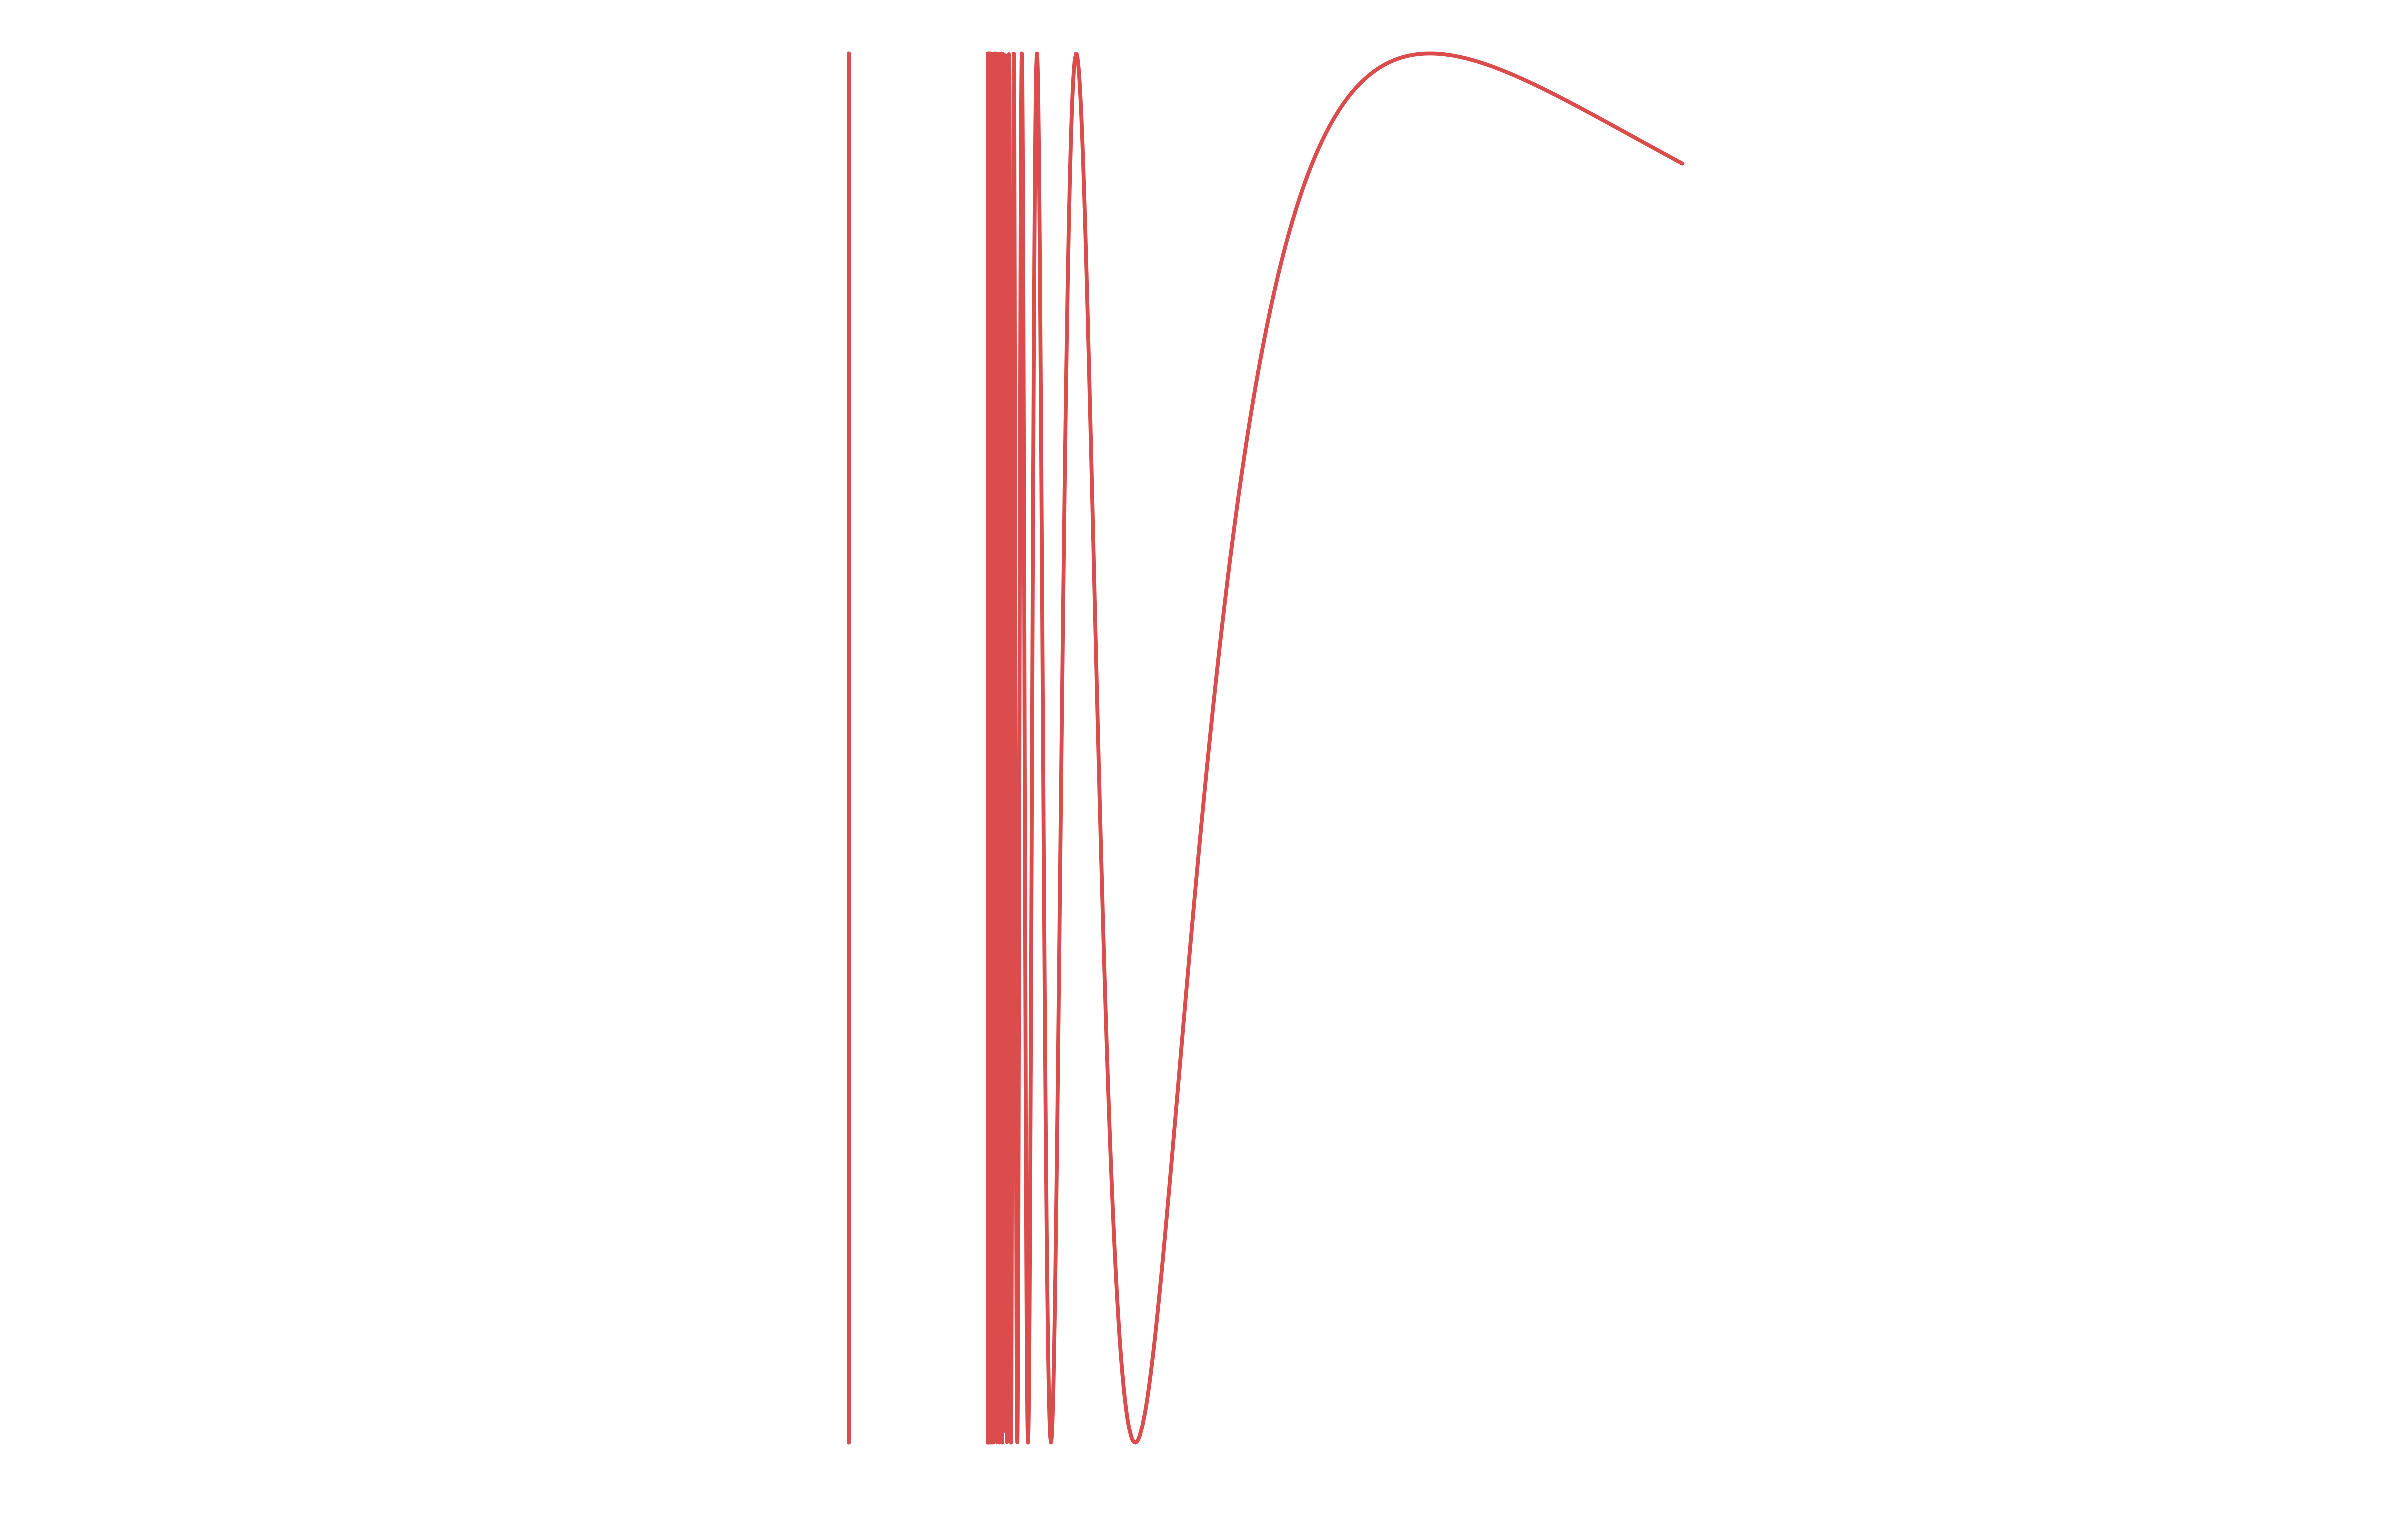
\includegraphics[scale = 0.2]{Figures/Chapter3/topologistsSineCurve.eps}
            \caption{The topologists Sine Curve, defined by $x \times \sin{\frac{1}{x}}$.}
            \label{fig_3.2}
        \end{figure}

        Let $S=\{x \times \sin{\frac{1}{x}}:0 < x \leq 1\}$. This is the image of the continuous map
        $x \rightarrow x \times \sin{\frac{1}{x}$ from $(0,1] \rightarrow \R^2$, Since $(0,1]$ is
            connected, then so is $S$. by theorem \ref{3.1.6}. We call $\cl{S}=S \cup (0 \times
            [-1,1])$ the \textbf{topologist's sine curve} (see figure \ref{fig_3.2}).

            Suppose that $f:[a,c] \rightarrow \cl{S}$ is a path begining at $0$ and ending at a
            point in  $S$. The set  $T=\{t \in \R:f(t) \in 0 \times [-1,1]\}$ is closed, so it has a
            largest element $b$. Then  $f$ is a path mapping  $b \rightarrow 0 \times [-1,1]$ and
            taking all other points to $S$. Suppose that  $[b,c]=[0,1]$ and let $f(t)=(x(t),y(t))$
            where $x(0)=0$, $x(t)>0$ and $y(t)=\sin{\frac{1}{x(t)}}$ for all $t>0$. For  $n \in
            \Z^+$, choose  $0<u<x(\frac{1}{n})$ such that $\sin{\frac{1}{u}}=(-1)^n$. By the
            intermediate value theorem, there are $0<t_n<\frac{1}{n}$ with $x(t_n)=u$. Then the
            sequence $\{t_n\} \rightarrow 0$, and $x(t_n)=(-1)^n$, which diverges; a contradiciton
            since $x(0)=0$ and $\{t_n\} \rightarrow 0$. Hence $\cl{S}$ is not path connected.

    \end{enumerate}
\end{example}
